%%% This LaTeX source document can be used as the basis for your technical
%%% report. Intentionally stripped and simplified
%%% and commands should be adjusted for your particular paper - title, 
%%% author, citations, equations, etc.
% % Citations/references are in report.bib 

\documentclass[conference]{acmsiggraph}

\usepackage{graphicx}
\graphicspath{{./images/}}
\newcommand{\figuremacroW}[4]{
	\begin{figure}[h] %[htbp]
		\centering
		\includegraphics[width=#4\columnwidth]{#1}
		\caption[#2]{\textbf{#2} - #3}
		\label{fig:#1}
	\end{figure}
}

\newcommand{\figuremacroF}[4]{
	\begin{figure*}[h] % [htbp]
		\centering
		\includegraphics[width=#4\textwidth]{#1}
		\caption[#2]{\textbf{#2} - #3}
		\label{fig:#1}
	\end{figure*}
}


\usepackage{lipsum}

\usepackage{xcolor}
\definecolor{lbcolor}{rgb}{0.98,0.98,0.98}
\usepackage{listings}

\lstset{
	escapeinside={/*@}{@*/},
	language=C,
	basicstyle=\fontsize{8.5}{12}\selectfont,
	numbers=left,
	numbersep=2pt,    
	xleftmargin=2pt,
	%numberstyle=\tiny,
	frame=tb,
	%frame=single,
	columns=fullflexible,
	showstringspaces=false,
	tabsize=4,
	keepspaces=true,
	showtabs=false,
	showspaces=false,
	%showstringspaces=true
	backgroundcolor=\color{lbcolor},
	morekeywords={inline,public,class,private,protected,struct},
	captionpos=t,
	lineskip=-0.4em,
	aboveskip=10pt,
	%belowskip=50pt,
	extendedchars=true,
	breaklines=true,
	prebreak = \raisebox{0ex}[0ex][0ex]{\ensuremath{\hookleftarrow}},
	keywordstyle=\color[rgb]{0,0,1},
	commentstyle=\color[rgb]{0.133,0.545,0.133},
	stringstyle=\color[rgb]{0.627,0.126,0.941},
}


\TOGonlineid{45678}
\TOGvolume{0}
\TOGnumber{0}
\TOGarticleDOI{1111111.2222222}
\TOGprojectURL{}
\TOGvideoURL{}
\TOGdataURL{}
\TOGcodeURL{}

\title{Temple on Mars}

\author{Zoe Wall \\\ 40182161@live.napier.ac.uk \\
Edinburgh Napier University \\
Computer Graphics (SET08116)}
\pdfauthor{Zoe Wall}

\keywords{skybox, hierarchy, lighting, OpenGL, GLSL}

\begin{document}

\teaser{
   \centering
   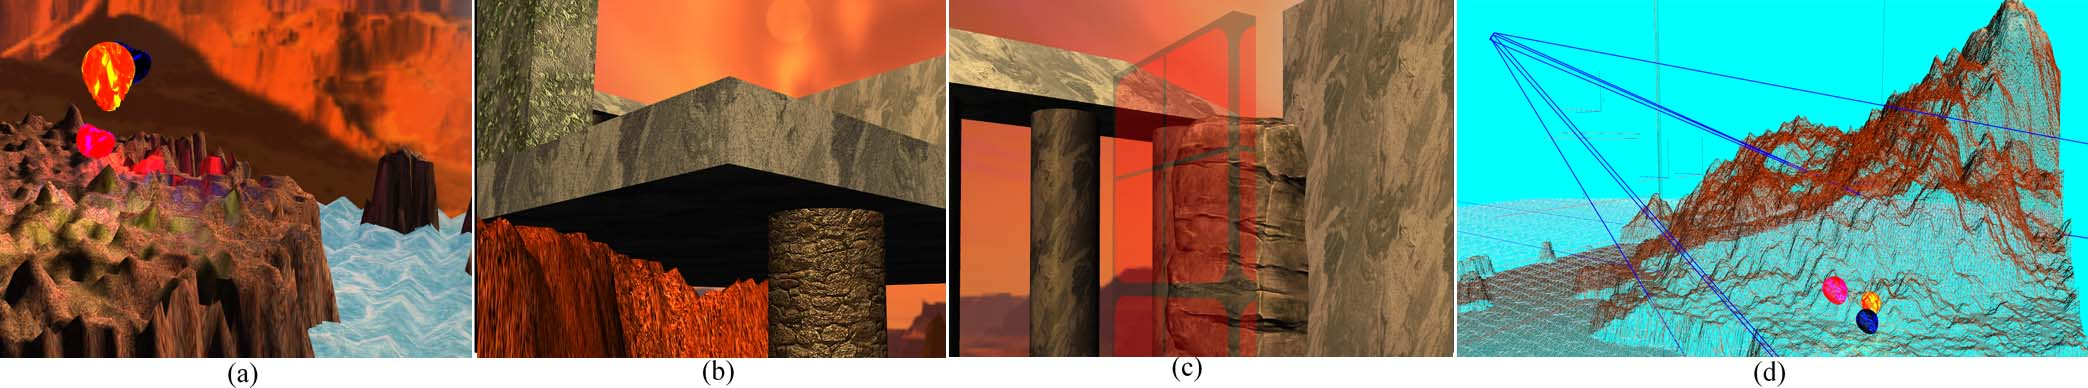
\includegraphics[width=1.0\textwidth]{images/teaser}
   \caption{Project screenshots. (a) Point lights with Vertex Displacement and Parent-Child Hierarchy, (b) Normal Mapping, (c) Transparency and Render Ordering, and (e) View Frustrum Culling and Wireframing.}
   \label{fig:teaser}
 }	

\maketitle

\begin{abstract}
This project aims to implement a 3D scene, rendered in real-time using OpenGL and C++. The project was intended to be aesthetically interesting, but more importantly intended to show an understanding of fundamental computer graphics principles. This report details the industry techniques used within the development of the outdoor Mars scene.
\end{abstract}

\keywordlist
%\copyrightspace

\section{Introduction}

\figuremacroW
{DestinyMars1}
{Project Inspiration - Destiny Mars Landscape}
{\protect\cite{Destiny}}
{1.0}

\paragraph{Project Aims}The main aims of this project were not to produce something photo-realistic but to show understanding of the key concepts of computer graphics. The setting of the scene is a form of landscape on Mars with the inclusion of some extra-terrestrial objects and strange effects. The initial ideas were that of a barren land filled with broken stone and large metallic structures, littered with weeds and with dust clouds. The main inspiration for this type of scene comes from the vast landscapes used within Destiny (see Figure \ref{fig:DestinyMars1}).

\paragraph{High Level of Detail} Using different texturing techniques, a high level of detail is hope to be achieved. For example normal mapping to give the impression of more shape and detail to an object. Along with blend mapping and alpha mapping used on different objects in the scene.

\figuremacroW
{fallout}
{Normal Mapping example - Fallout 4}
{\protect\cite{Fallout4}}
{1.0}

Even with the improvements to GPU hardware in recent times, there is always a need for optimisation. In this scene optimisation techniques such as a scene graph for spacial partitioning was used alongside view culling.

\section{Implementation}

\subsection{Parent-Child Hierarchy}

A scene graph in the form of a parent-child hierarchy was implemented within the scene to partition the scene's space into smaller parts to allow for optimization and easier control over the overall development of the scene. The scene graph contains all of the geometry for the particular scene, it makes transformations and rendering easier as a parent-child hierarchy is such that every object in the scene inherits from a single root. This means that each child object's own model matrix is relative to it's parent's (see Listing \ref{lst:hierarchy}).

\begin{lstlisting}[label = {lst:hierarchy}, caption={Parent-child Hierarchy Update Method}]
 	if (parent){
		if (parent->myType != sky && myType != sky)
		{
			mworld = parent->mworld * mlocal;
		}
	}

	for (auto &e : children)    // iterate through list of children
	{
		Obj* child = e.second;
		child->normalMatrix = normalMatrix;  // set normal matrix for child object 
		child->update(this, delta_time);     // recurse
	}
\end{lstlisting}

This technique is not only useful for positioning the geometry into world space, it is also useful for rendering and culling. For example, a test can be made to see if an object's parent is not visible within the view frustrum, then it should assume that the child is also not visible and continue without performing the calculations.
Rendering and updating is done by traversing the n-tree that makes up the hierarchy. Firstly the root is rendered if visible. It then iterates through a list of it's children rendering each in turn. If a child of the root is invisible, it will not check to see whether the children are, and the whole branch will be culled. 

\subsection{Lighting}
Lighting in computer graphics is very important to get correct as it is the main basis of making a scene look realistic. Lighting calculations are performed on the GPU by programs called shaders. There are three programmble shaders within the graphics pipeline: the vertex, the geometry and the fragment shader.
    There are two main methods for lighting a scene using OpenGL: Gouraud shading, and Phong shading.
Gouraud shading is %% quote here! 
calculations performed per geometry vertex. This means that an object in a scene is coloured by interpolating the colour value between each vertex, as opposed to the more expensive but better Phong shading. Where colour calculations are performed on the fragment shader on a per pixel basis. (See Figure \ref{fig:gouraudPhong})

\figuremacroW
{gouraudPhong}
{Implementation of both Gouraud and Phong shading within the project. }
{The sphere on the left is Gouraud shaded, note the specular reflection is less concentrated and accurate, whilst the sphere on the right is Phong shaded.}
{1.0}

The main lighting types used within the scene:
\begin{itemize}
    \item {Ambient} Constant lighting which is representative of light from a fixed-intensity and fixed-coloured source. It is used to raise the overall brightness level of every object within the scene. 
    \item {Diffuse} Directional lighting, percentage brightness according to the angle of the light and vertex.
    \item {Specular} Reflective lighting, what makes an object appear to be shiny or reflective.
    \item {Attenuation} Light from a source that degrades over distance such as a point or a spot light.
\end{itemize}

The equation for ambient lighting is as follows:
\begin{equation} \label{ambientLightingEq}
    DA
\end{equation}
where $D$ is the diffuse reflection of the material and $A$ is the ambient intensity of the scene. The diffuse reflection is the coloured reflection component of the material.

Diffuse lighting is a little more complex as the intensity of the light is not constant. It relies on the direction of the light source to the normal of the geometry. In simple Gouraud shading, the transformed normal of each vertex is calculated, and the angle between that and the light direction is calculated using the scalar product. If the vertex is facing the light source, the intensity of the light will be 100\% and however, 90 degrees away from the light, the intensity drops to zero.

\begin{equation} \label{diffuseLightingEq}
    DA max(L N, 0)
\end{equation}

Specular lighting is dependent on the object's material. It is the bright highlight that is dependent on the direction of the eye, in this case the position of the camera. How reflective the material is depends on how bright and how large this highlight appears on the object. In computer graphics it is a very important element in creating a realistic lighting model, as it mimics the reflective properties of a surface. %% reorder
For this calculation, the position of the eye (or camera) must also be taken into account. 

\begin{equation}
    SC max(H N, 0)^m
\end{equation}

where:

\begin{equation} 
    V = \frac{eyePosition - worldPosition}{||eyePosition - worldPosition||}
\end{equation}

Where the eye Positon is the position of the camera, and the world position is the position of the vertex in world space, and H is the half vector, V plus the direction of the light normalised.

Attenuation lighting is where the lighting is taken from a point source or a spot source, where the intensity is multiplied by a factor of its range. In the real world lighting model, light from a point source drops off exponentially, however attenuation values are set for artistic purposes, to give a more even fall off. 

\subsection{Texturing}

\subsection{Terrain Generation}

\subsubsection{Vertex Displacement}

%% jereome
%%Textures used for vertex displacement 
Vertex Displacement Mapping or simply Displacement Mapping is a technique allowing to deform a polygonal mesh using a texture (displacement map) in order to add surface detail. The scene includes a procedurally generated terrain from a height map %% change this

\subsubsection{Normal Mapping}
%% talk about difference between bump mapping and how normal mapping is better
\figuremacroW
{normalMap}
{Normal Mapping Example from Scene}
{These pillars are completely smooth cylinder objects, however note how by using a normal map, another level of detail is added making it appear that the pillars are made from stone, with cracks and bumps.}
{1.0}

\subsubsection{Skybox}
A skybox is essentially a set of textures called a cubemap. These are seamless textures that fit together like a layout of a cube
A skybox is a cube rendered from the inside out, with the depth buffer turned off. It also needs to be transformed with the camera, so it gives the effect that it is infinitely large and far away.

\subsubsection{Transparency}

To render a transparent object, OpenGL has a mechnaism called blending, which combines any colour already in the frame buffer with the colour of the primitive, and the resulting blended colour is stored back in the framebuffer \cite{openGLBlend}. This causes problems for rendering a scene in real-time as render order must be taken into account. This is because if the transparent object is rendered first, the texture behind the object is blended to it, which means that any object rendered after the glass will be occluded by the object.
To solve this issue, an enumeration was used to check for object type when rendering. If the object rendered is a glass object it is rendered separately after the main render function.

\section{Post-Processing}

%% add definition of post processing here
Post-processing is defined as any rendering technique that is applied after the initial render. These techniques therefore require multiple render passes to different targets. For displaying to the screen, a vertex buffer object is created to use as a render target for the first pass; the scene is rendered normally to this frame buffer then the render target is set back to the screen. For the second render pass, a post process can be applied using the output from the first pass as a texture which is mapped to a screen quad.

\subsection{Greyscale}

For a grey scale effect, the colour is sampled from a texture of the first render pass. The final colour output is calculated by the dot product of the sampled colour and a greyscale intensity value.

\figuremacroW
{greyscale}
{A screen capture of the scene rendering in greyscale}
{This is rendered as a black and white texture mapped to a screen quad.}
{1.0}

\subsection{Vignette}

A vignette is a loss in clarity and brightness towards the corners of the screen. This effect was created by calculating a radial black and white gradient. The product of this gradient factor and the sampled colour from the original render pass resulted in an output with darker edges. The gradient was achieved by calculating the length of a vector from the screen quad's centre position to the current fragment position, this length was inverted and used as a factor to scale the sampled colour. 

\begin{lstlisting}[label = {lst:vignette}, caption={Fragment Shader Code Snippet for Vignette Calculation}]
void main()
{
	// Sample texture colour
	vec4 colourSample = texture(tex, tex_coord);

	// calculate the position vector for current pixel
	vec2 position = (gl_FragCoord.xy / resolution) - vec2(0.5);

	// get factor
	float len = length(position);
	len = 1.0 - len;

	colourSample *= len; // multiply output by inverted length

	colour = vec4(colourSample.rgb, 1.0);
}
\end{lstlisting}

To calculate the position vector, gl_FragCoord was used, a built in
The length is inverted due to the RGB colour model being additive, meaning that a value of zero for each component will result in black, the shortest lengths are the coordinates closer to the centre of the screen, however multiplying a smaller number to the sampled colour would have produced the opposite effect.

\subsection{Shadows}

\subsection{Blur}

\subsection{Bloom}

\section{Advanced Rendering Techniques}

\subsection{Graphical User Interface}

A GUI was implemented for easier control over the post processing effects. 

\subsection{Particles}

To create a particle effect the geometry shader is used. twice. report is good. 


\subsection{Optimization}

\subsubsection{Profiling}
Originally, with no optimisation techniques implemented, running the performance profiler within Visual Studio 2013 showed that the most expensive call path based on the sample counts was the render() function called to traverse down the hierarchy and render each object in turn.

\figuremacroW
{compare}
{Comparison of Profiling Results}
{The results on the left are after optimization, it shows the hot path render() to be roughly 20\% lower than the original results.}
{1.0}

The rendering function initially used 83.20\% of inclusive samples, meaning it was the most expensive function overall. After applying the optimisation techniques, the profiler returned 63.9\% for the main render function meaning the frustrum culling saved on average 20\% of the program's performance. This can also be noted when monitoring the frame-rate for the scene, with the frame-rate clipped, the frame-rate stays at a constant 60FPS. Features such as exploring the environment, and toggling wire-frames on and off make no impact on this frame-rate whatsoever. When running without a clip, the frame rate can be seen to improve when looking away from a complex part of the scene which shows that the view clipping is working, as there is less operations per frame and therefore an improved frame-rate. The slowest parts of the code apart from the render function are part of the geometry builder in the setup of the scene. There is a peak at the start of the program of CPU usage. Further analysis shows that the the hot paths here are both the function to generate the terrain, and the function generating the plane for the water mesh. In both cases, the functions are expensive due to the high number of polygons required to make the mesh look realistic. 


\subsubsection{Geometry Shader For Debugging}
%%calculate bounding sphere %%show radius algorthim here
The geometry shader is the second part of the graphics pipeline. Unlike the vertex or fragment shaders, the geometry shader is used to transform the actual geometry of an object. A primitive is passed through the shader. For example a point, and the geometry shader can add or remove vertices. In the scene, the geometry shader was used to draw the radius of the bounding spheres for each object in the hierarchy. Each mesh has a selection of positions on the vertex array buffer, to calculate the radius a function iterates through positions to find the largest point of the geometry, the length of this as a float is passed into the geometry shader along with the center point, and a line is drawn.

\subsubsection{View Frustrum Culling}
%% RTR
View frustum culling is an important optimisation technique which means removing objects that are out of view. By calculating the frustrum planes of the camera, intersection tests can be performed to see if an object's bounding volume is within view. Any object that is classified as outside of the view frustrum is culled - not rendered. In the scene the intersection tests are performed using bounding spheres. The use of bounding spheres as volumes is limited due to the fact most objects within the scene are not spheres. However this is a reasonable enough approximation to use. Although it has drawbacks, it is also less expensive to compute, as it is only a centre point test for each plane. The plane equation is used to test which side the 

\section{Conclusion}
In conclusion, the first attempt at building up the basics of the mars scene was successful. It showed many core principles of computer graphics, in particular optimisation techniques with view frustrum culling, and texturing effects for more than just basic decoration. Future work will be to further the lighting and optimisation techniques to recreate light more realistically. For example to show how light bends as it passes through a transparent object, and use Screen Space Ambient Occlusion to add further level of detail.
\bibliographystyle{acmsiggraph}
\bibliography{report}


\end{document}